\documentclass[main.tex]{subfiles}

\begin{document}

\subsection{Secondo esercizio}
\includegraphics[width=\textwidth]{2015-2207-2.jpg}

Per il sistema rappresentato in figura, soggetto alla sola forza attiva $\vec{F}$, applicata in direzione verticale nel punto B, si chiede di calcolare:

\begin{enumerate}
	\item Le reazioni vincolari a terra in A e D.
	\item Le azioni interne nell’asta AC.
\end{enumerate}

\subsection{Soluzione secondo esercizio}

\subsubsection{Osservazioni importanti}

\begin{enumerate}
	\item Il sistema è composto da un corpo rigido, l'asta AC, e due vincoli: una biella (o pendolo semplice) DC e un carrello in A.
	\item Una biella trasmette unicamente la reazione assiale.
	\item La biella è ad un angolo pari a $\frac{3\pi}{4}$, per cui le componenti orizzontali e verticali di $R_C$ saranno uguali.
\end{enumerate}

\subsubsection{Verifica preliminare di isostaticità}
Verifico che $gdl_{tot} = gdv_{tot}$:
\begin{figure}[H]
  \begin{subfigure}[b]{.5\textwidth}
  \centering
  \[
  	gdv: \begin{cases}
		gdv_{biella} = 1\\
		gdv_{carrello} = 2
  	\end{cases}
  \]
  \caption{Gradi di vincolo del sistema.}
  \end{subfigure}
  \hfill
  \begin{subfigure}[b]{.5\textwidth}
  \centering
  \[
  	gdl: \begin{cases}
  		gdl_{asta} = 3\\
  	\end{cases}
  \]
  \caption{Gradi di libertà del sistema.}
  \end{subfigure}
  \caption{Verifica preliminare di isostaticità.}
\end{figure}

\subsubsection{Primo punto}
\begin{figure}[H]
\centering
\resizebox{.5\textwidth}{!}{% First image 2015 06 29

\begin{tikzpicture}

  \tiny

  \point{h}{-1}{0};
	\point{a}{0}{0};
  \point{b}{1}{0};
  \point{c}{2}{0};

  \beam{2}{a}{c}

  \load{1}{b}[90]

  \load{1}{c}[135]

  \load{1}{a}[180]

  \load{2}{a}

  \notation{1}{a}{A}[below];
  \notation{1}{b}{B}[below];
  \notation{1}{c}{C}[below];

  \notation{1}{a}{$M_A$}[above];
  \notation{1}{h}{$H_A$}[above right];
  \notation{1}{b}{$F$}[above right];
  \notation{1}{c}{$R_C$}[above right];

  %  \notation{1}{b}{B}[above left];
  %  \notation{1}{c}{C}[above=0.1];
  %  \notation{1}{d}{D}[above right];
  %  \notation{1}{e}{E}[above right];
  %  \notation{1}{f}{$\vec{F}$}[above right];

  %  %Degrees
  %  \notation{1}{a}{$\frac{\pi}{3}$}[above right=0.325];
  %  \notation{1}{e}{$\frac{\pi}{3}$}[above left=0.325];

\end{tikzpicture}}
\caption{Reazioni vincolari nell'asta AC}
\end{figure}

\[
	\begin{cases}
		H_A + R_{x_C} = 0\\
		F + R_{y_C} = 0\\
		M_A - LF - 2LR_{y_C} = 0\\
		R_{x_C} = R_{y_C}
	\end{cases}
	\Longrightarrow
	\begin{cases}
		H_A = -R_{x_C}\\
		F = -R_{y_C}\\
		M_A = LF - 2LF = -LF\\
		R_{x_C} = R_{y_C}
	\end{cases}
	\\
	\Longrightarrow
	\begin{cases}
		H_A = F\\
		M_A =  -LF\\
		R_{y_C}= -F\\
		R_{x_C} = -F
	\end{cases}
\]

Alcune reazioni vincolari risultano negative, per cui è stato scelto la direzione inversa rispetto a quella reale. Per cui correggiamo il grafico:

\begin{figure}[H]
\centering
\resizebox{.5\textwidth}{!}{\input{chapters/2/2015/2207/2/reazioni_corrette_asta_AC.tex}}
\caption{Reazioni vincolari nell'asta AC corrette}
\end{figure}

Le reazioni vincoli in A e in D risultano quindi, col grafico corretto:

\begin{figure}[H]
  \begin{subfigure}[b]{.5\textwidth}
  \centering
  \[
  	A: \begin{cases}
		H_A = F\\
		M_A = LF
  	\end{cases}
  \]
  \caption{Reazioni vincolari in A.}
  \end{subfigure}
  \hfill
  \begin{subfigure}[b]{.5\textwidth}
  \centering
  \[
  	D: \begin{cases}
  		R_{x_D} = F\\
  		R_{y_D} = F
  	\end{cases}
  \]
  \caption{Reazioni vincolari in D.}
  \end{subfigure}
  \caption{Reazioni vincolari richieste dal primo punto.}
\end{figure}

\subsubsection{Secondo punto}
\paragraph{Sforzo normale}

\begin{figure}[H]
\centering
\resizebox{.5\textwidth}{!}{\input{chapters/2/2015/2207/2/sforzo_normale.tex}}
\caption{Sforzo normale nell'asta AC}
\end{figure}

Lo sforzo normale nell'asta AC è di \textbf{compressione}, per cui per convenzione è negativo.

\begin{figure}[H]
\centering
\resizebox{.5\textwidth}{!}{% First image 2015 06 29

\begin{tikzpicture}

  \tiny

  \point{h}{-1.2}{0};
  \point{a}{0}{0};
  \point{b}{1}{0};
  \point{c}{2}{0};
  \point{d}{3.2}{0};

  \beam{2}{a}{c}

  % \load{1}{b}[90]

  % \load{1}{d}[180]

  % \load{1}{h}

  % \load{2}{a}

  % \notation{1}{a}{A}[below];
  % \notation{1}{b}{B}[below];
  % \notation{1}{c}{C}[above];

  % \notation{1}{a}{$M_A$}[above];
  % \notation{1}{h}{$H_A$}[above right];
  % \notation{1}{b}{$F$}[above right];
  % \notation{1}{d}{$R_{x_C}$}[above left];

  %  \notation{1}{b}{B}[above left];
  %  \notation{1}{c}{C}[above=0.1];
  %  \notation{1}{d}{D}[above right];
  %  \notation{1}{e}{E}[above right];
  %  \notation{1}{f}{$\vec{F}$}[above right];

  %  %Degrees
  %  \notation{1}{a}{$\frac{\pi}{3}$}[above right=0.325];
  %  \notation{1}{e}{$\frac{\pi}{3}$}[above left=0.325];

  \internalforces{a}{c}{1}{1}[0][blue];

\end{tikzpicture}}
\caption{Grafico sforzo normale nell'asta AC}
\end{figure}

\paragraph{Taglio}

\begin{figure}[H]
\centering
\resizebox{.5\textwidth}{!}{% First image 2015 06 29

\begin{tikzpicture}

  \tiny

  \point{a}{0}{0}
  \point{c}{1}{0}
  \point{b}{2}{2}
  \point{d}{1}{1}

  \beam{2}{a}{b}

  \internalforces{a}{d}{2.121}{2.121}[0][blue];
  \internalforces{d}{b}{-0.707}{-0.707}[0][red];

\end{tikzpicture}}
\caption{Taglio nell'asta AC}
\end{figure}

Il taglio nell'asta AC impone una rotazione \textbf{anti-oraria}, per cui per convenzione è negativo.

\begin{figure}[H]
\centering
\resizebox{.5\textwidth}{!}{% First image 2015 06 29

\begin{tikzpicture}

  \tiny

  \point{a}{0}{0}
  \point{e}{2.5}{-0.866}
  \point{b}{0.5}{0.866}
  \point{d}{1.5}{0.866}
  \point{c}{1}{2*0.866}

  \beam{2}{a}{c}

  \internalforces{a}{b}{0.866}{0.866}[0][blue];
  \internalforces{b}{c}{-1.732}{-1.732}[0][red];

\end{tikzpicture}}
\caption{Grafico taglio nell'asta AC}
\end{figure}

\paragraph{Momento flettente}

Le fibre tese sono nella parte inferiore del grafico.

\begin{figure}[H]
\centering
\resizebox{.5\textwidth}{!}{% First image 2015 06 29

\begin{tikzpicture}

  \tiny

  \point{a}{0}{0}
  \point{e}{2.5}{-0.866}
  \point{b}{0.5}{0.866}
  \point{d}{1.5}{0.866}
  \point{c}{1}{2*0.866}

  \beam{2}{a}{c}

  \internalforces{a}{b}{0.5*1.732}{-1.732}[0][red];
  \internalforces{b}{c}{-1.732}{0}[0][red];

\end{tikzpicture}}
\caption{Grafico del momento flettente nell'asta AC}
\end{figure}

\end{document}